\chapter{Simulation Results}

This chapter contains simulation results demonstrating and comparing the capabilities of the baseline and adaptive controllers when applied to the nonlinear evaluation model as depicted in Figure~\ref{fig:simblockdiagram}.
Before presenting the simulation studies showing the response of the vehicle to different commanded trajectories, some additional uncertainties which were used in the simulations are first outlined.

\begin{figure}[h]
  \fontsize{11pt}{11pt}\selectfont
  \begin{center}
    \begin{tikzpicture}[auto, scale=0.75, every node/.style={transform shape}, node distance=1.0cm, >=latex']
      \node[squareblock, minimum height=1cm, minimum width=2cm] (block1){Baseline};
      \node[squareblock, below of=block1, node distance=1.5cm, minimum height=1cm, minimum width=2cm] (block2){Adaptive};
      \matrix[ampersand replacement=\&, row sep=0.5cm, left of=block1,node distance=1cm] (block1in) {%
      \node [coordinate] (b1inA) {};\\
      \node [coordinate] (b1inB) {};\\
      };
      \matrix[ampersand replacement=\&, row sep=0.5cm, left of=block2,node distance=1cm] (block2in) {%
      \node [coordinate] (b2inA) {};\\
      \node [coordinate] (b2inB) {};\\
      };
      \node [left of=b2inB, node distance=0.5cm] (2B) {};
      \node [below of=2B, node distance=0.12cm] (2B2) {};
      \node [left of=b2inA, node distance=1.0cm] (2A) {};
      \node [below of=2A, node distance=0.12cm] (2A2) {};
      %
      \node[whitesum,right of=block1, node distance=2.0cm] (sum1) {};
      \node[squareblock, minimum height=1cm, minimum width=1.0cm, label=below:{delay}, right of=sum1,node distance=1.5cm] (block3) {$\tau$};
      \node[squareblock, minimum height=1cm, minimum width=1.0cm, label=below:{\shortstack[c]{Actuator\\Dynamics}}, right of=block3,node distance=2.5cm, inner sep= 1mm] (block4) {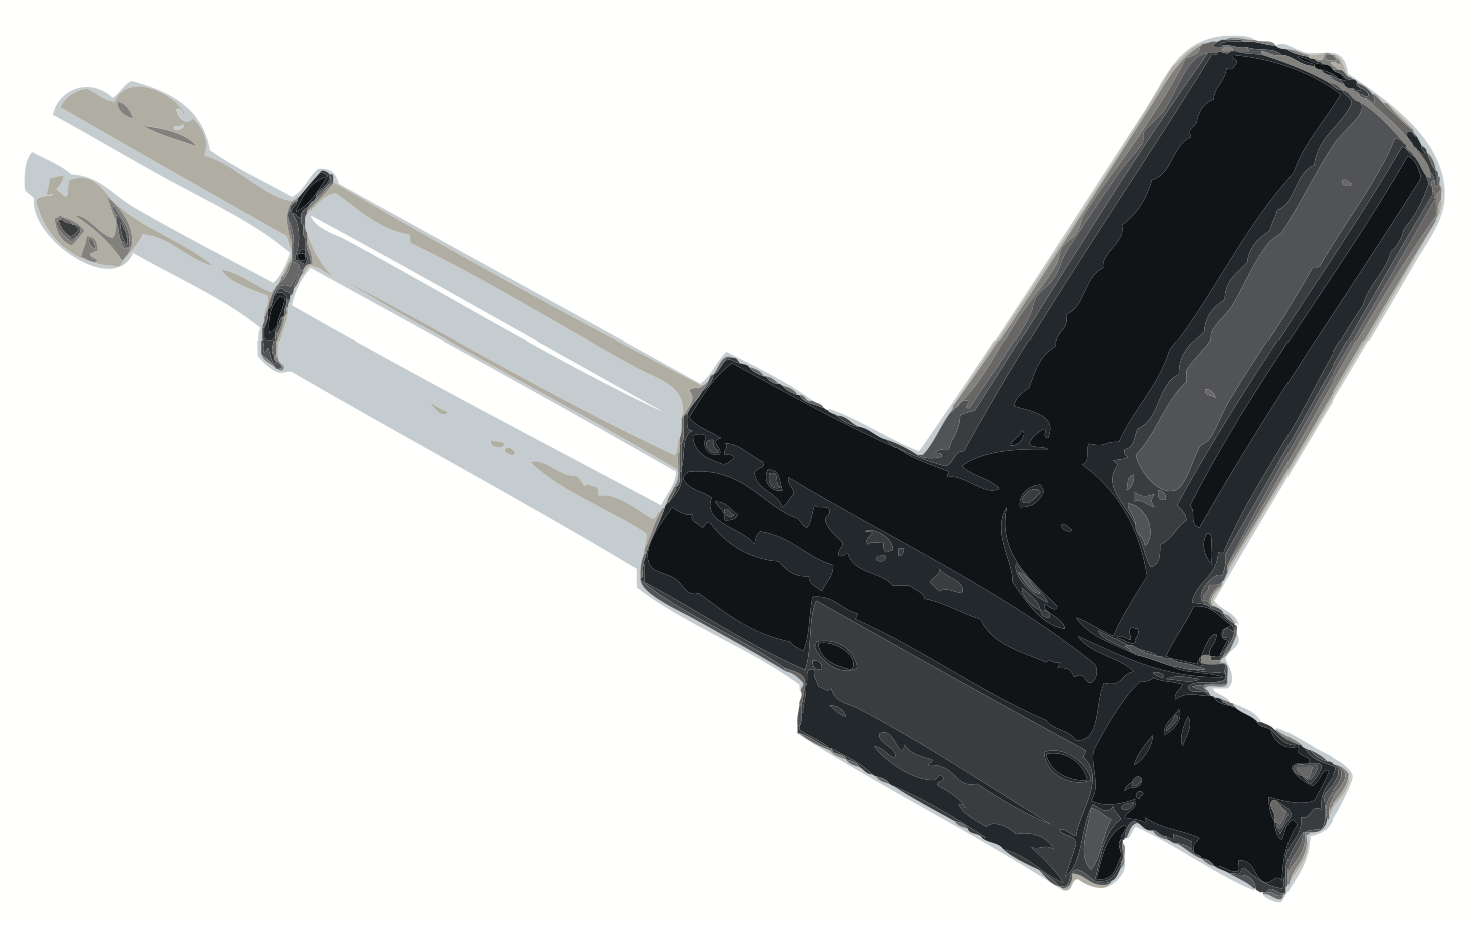
\includegraphics[width=1.6cm]{\figurepath/actuator_image.png}};
      \node [right of=block4,draw=black, anchor=west,node distance=2.0cm, label=below:{\shortstack[c]{Equations of\\Motion}}, minimum width=2cm, inner sep= 0mm] (block5) {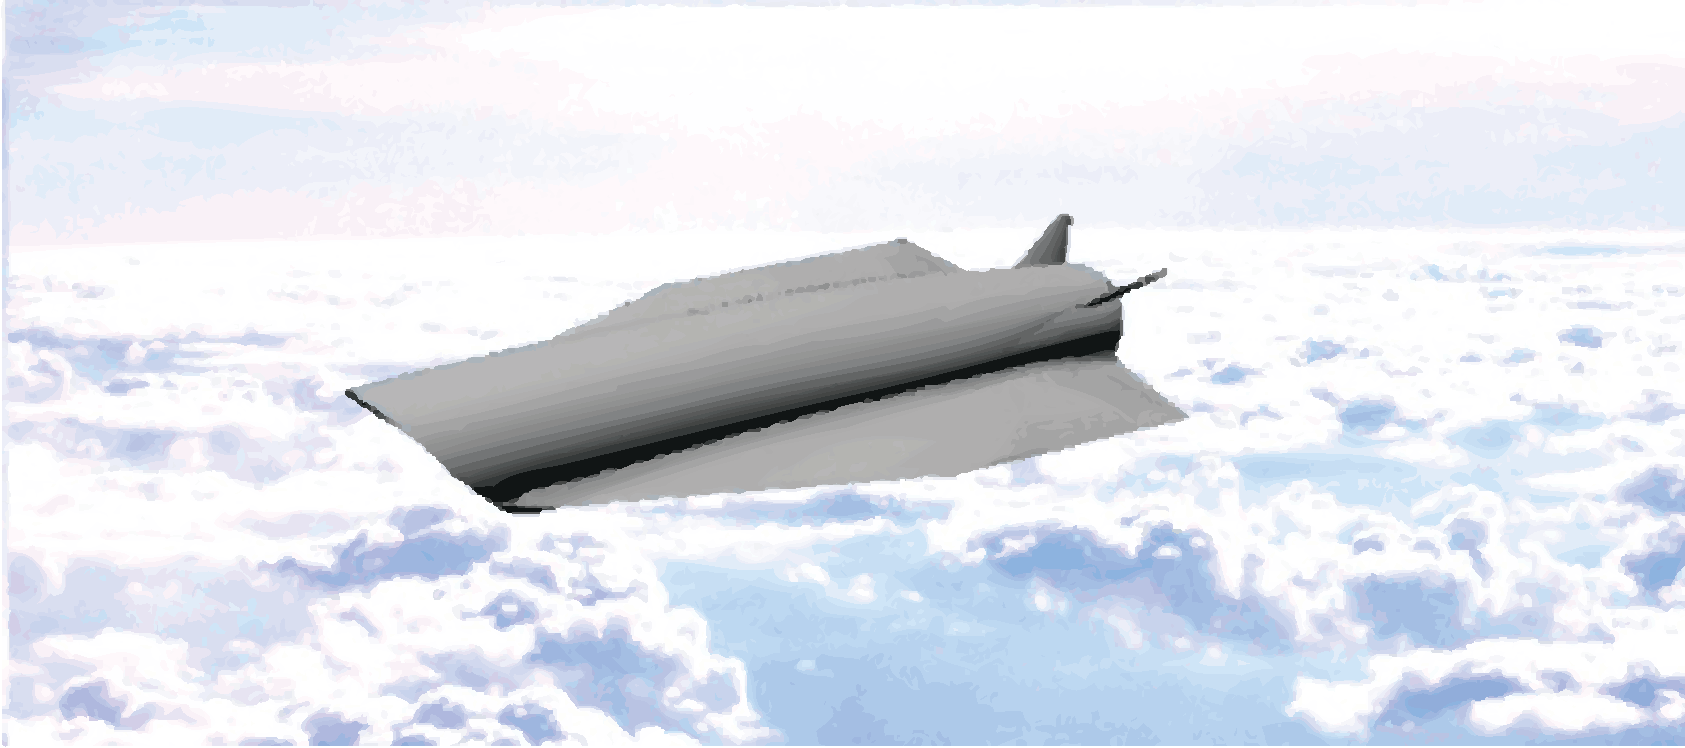
\includegraphics[width=4cm]{\figurepath/ghvclouds.pdf}};
      \node[whitesum,right of=block5, node distance=3.0cm] (sum2) {};
      \node[squareblock, minimum height=1cm, minimum width=1.0cm, right of=sum2,node distance=1.5cm] (block6) {ZOH};
      \node[squareblock, minimum height=1cm, minimum width=1.0cm, right of=block6,node distance=1.6cm] (block7) {Filter};
      \node[output, right of=block7,node distance=1.5cm] (output1) {};
      \node[input, below of=block2,node distance=1.0cm](input2){};
      \node[input, above of=sum2,node distance=1.0cm](input3){};
      \draw [->]  (b1inA) + (-2.5cm,0cm) -> node [pos=0.15]{$z_{\text{cmd}}$}  (b1inA);
      \draw [->]  (b1inB) + (-0.5cm,0cm) -> (b1inB);
      \draw [->]  (b2inA) + (-1cm,0cm) -> (b2inA);
      \draw [->]  (b2inB) + (-2.0cm,0cm) -> node[name=TB,node distance=2.5cm]{} (b2inB);
      \draw[->](block7) --  node[name=yi,pos=0.5]{} (output1);
      \draw[-](yi) |- (input2);
      \draw[-](b1inB) + (-0.5cm,0cm) -- (2B2);
      \draw[-](b1inA) + (-1.0cm,0cm) -- (2A2) ;
      \draw[-] (b2inB) + (-2.0cm,0cm) |- (input2);
      \draw[->](block1) -- (sum1);
      \draw[->](block2) -| (sum1);
      \draw[->](sum1) -- (block3);
      \draw[->](block3) -- (block4);
      \draw[->](block4) -- (block5);
      \draw[->](block5) -- (sum2);
      \draw[->](sum2) -- (block6);
      \draw[->](block6) -- node[name=azoh,pos=0.4]{} (block7);
      \draw[->](input3) -- (sum2);
      %
      \begin{pgfonlayer}{background}
        \path (block1 |- block1)+(-2.5,0.7) node (c) {};
        \path (block2 -| block2)+(2.5,-0.7) node (d) {};
        \path[fill=gray!20, draw, dashed] (c) rectangle (d);
      \end{pgfonlayer}
      %
      \begin{pgfonlayer}{background}
        \path (block6 |- block6)+(-0.9,0.7) node (c) {};
        \path (block7 -| block7)+(0.9,-0.7) node (d) {};
        \path[fill=gray!20, draw, dashed] (c) rectangle (d);
      \end{pgfonlayer}
      \node [above of=block1, node distance = 0.9cm] {100 Hz};
      \node [above of=azoh, node distance = 0.8cm] {600 Hz};
      \node [above of=sum2, node distance = 1.2cm] {noise};
    \end{tikzpicture}
    \caption{Simulation block diagram\label{fig:simblockdiagram}}
  \end{center}
\end{figure}

\section{Additional Uncertainties}

\subsubsection*{Sensor Bias/Noise}

Gaussian white noise was injected into the control loop as shown in Figure~\ref{fig:simblockdiagram}.
The variance of the noise used for each of the different sensor types is shown in Table~\ref{tab:noise}.
Each of these signals were passed through the first order navigation filter model, and fed back to the controller.
The filtered and unfiltered signals are shown in Figure~\ref{fig:noise}.
Additionally, sensor bias was added on feedback of the sideslip angle measurement, as is common to occur in inertially derived incidence measurements.

\begin{table}[H]
  \centering
  \caption{Noise variance\label{tab:noise}}
  \small
  \begin{tabular}{llr}
    \toprule
    Sensor type & Units & Variance \\
    \midrule
    Airspeed & [ft/s] & 1 \\
    Incidence & [rad] & 1e-6 \\
    Angular Rate & [rad/s] & 1e-5 \\
    Euler Angles & [rad] & 1e-6 \\
    Altitude & [ft] & 10 \\
    \bottomrule
  \end{tabular}
\end{table}

\begin{figure}[H]
  \begin{center}
    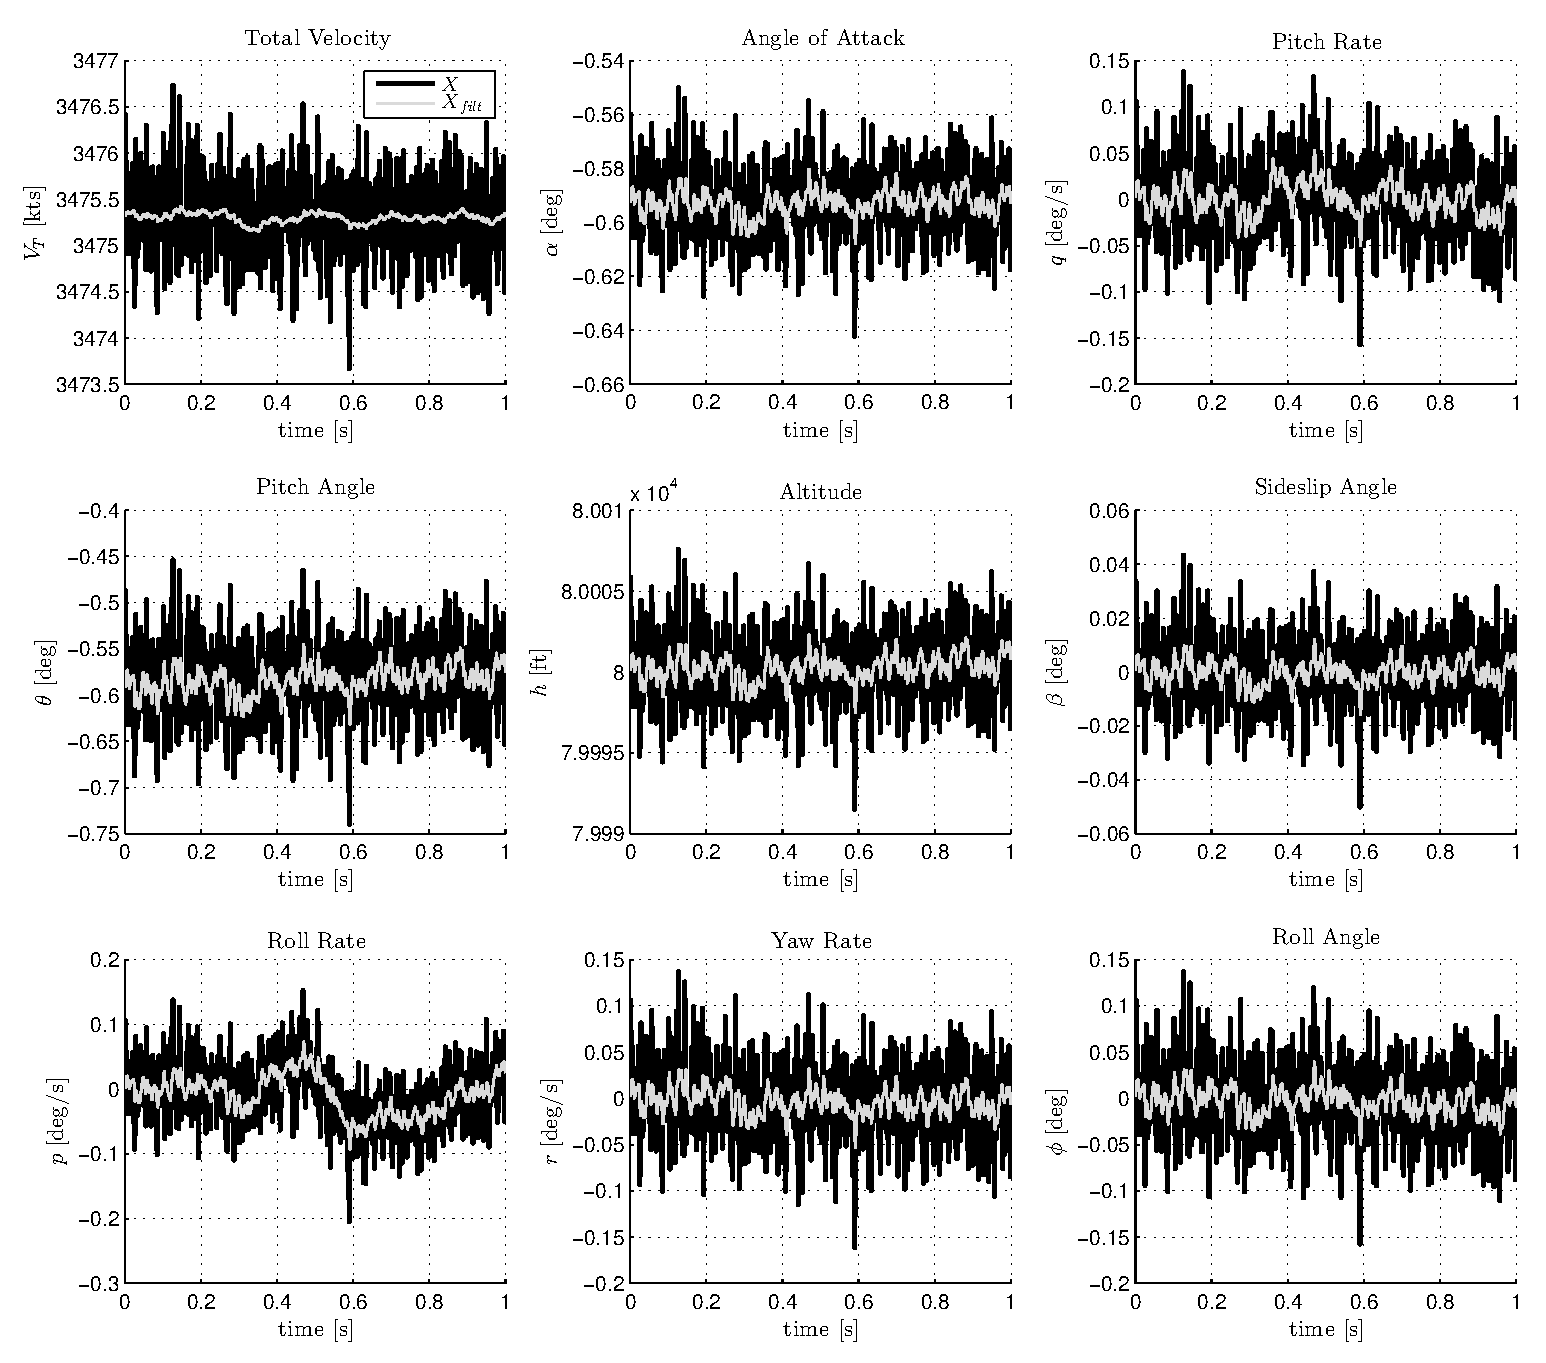
\includegraphics[width=5.0in]{\figurepath/filtervstate.eps}
    \caption{State measurements before and after navigation filter\label{fig:noise}}
  \end{center}
\end{figure}

\subsubsection*{Time Delay}

A input time delay was included in the simulation block diagram.
This time delay was set to zero when generating all of the simulation results shown in task 1 and task 2 below.
To empirically determine the input time delay margin of the different adaptive control strategies this time delay was varied during simulation until stability could not be maintained when flying a given trajectory.
The largest time delay which the system could tolerate while maintaining stability was recorded as the time delay.
However, since the ability of the controller to stabilize the system is dependent on the maneuver performed, these values are useful mostly for comparing the baseline and different adaptive controllers, as opposed to determining an actual delay margin for a given adaptive system.

\section{Results}

This section contains several simulation studies demonstrating the performance of both the baseline, ORM, and CRM adaptive controller in response to some of the uncertainties described above.
Two particular maneuvers are demonstrated below.
Task 1 is an angle of attack doublet command which begins from steady level cruise at Mach 6, followed by a +3 degree angle of attack command for 4 seconds, then -3 degree command for another 4 seconds, and back to steady level cruise.
Task 2 again begins at steady level cruise, and commands an 80 degree roll step.
Four uncertainties are considered for these two tasks:
\begin{enumerate}[label=\Alph*),itemsep=2pt,parsep=2pt,topsep=0pt,partopsep=0pt] % chktex 9 chktex 10
  \item{Control surface effectiveness}
  \item{Longitudinal CG shift}
  \item{Pitching moment coefficient $C_{m_{\alpha}}$}
  \item{Sensor bias on sideslip measurement}
\end{enumerate}
Each response will be denoted by the task number and letter corresponding to the uncertainty which it is subject to.
For example, 1B corresponds to task 1 with uncertainty B.
The components of the state trim vector $X_{\text{eq}}$ are shown in Table~\ref{tab:trimstate}.

\begin{table}[H]
  \centering
  \caption{Components of trim state vector at nominal flight condition of Mach 6}
  \small
  \begin{tabular}{llr}
    \toprule
    State variable & Units & Value \\
    \midrule
    $V_{T}$ & [ft/s] & 5866 \\
    $\alpha$ & [deg] & -0.59 \\
    $q$ & [deg/s] & 0 \\
    $\theta$ & [deg] & -0.59 \\
    $h$ & [ft] & 80,000 \\
    $\beta$ & [deg] & 0 \\
    $p$ & [deg/s] & 0 \\
    $r$ & [deg/s] & 0 \\
    $\phi$ & [deg] & 0 \\
    \bottomrule
  \end{tabular}\label{tab:trimstate}
\end{table}

\subsection{Task 1: Angle of Attack Doublet}

\begin{figure}[H]
  \begin{center}
    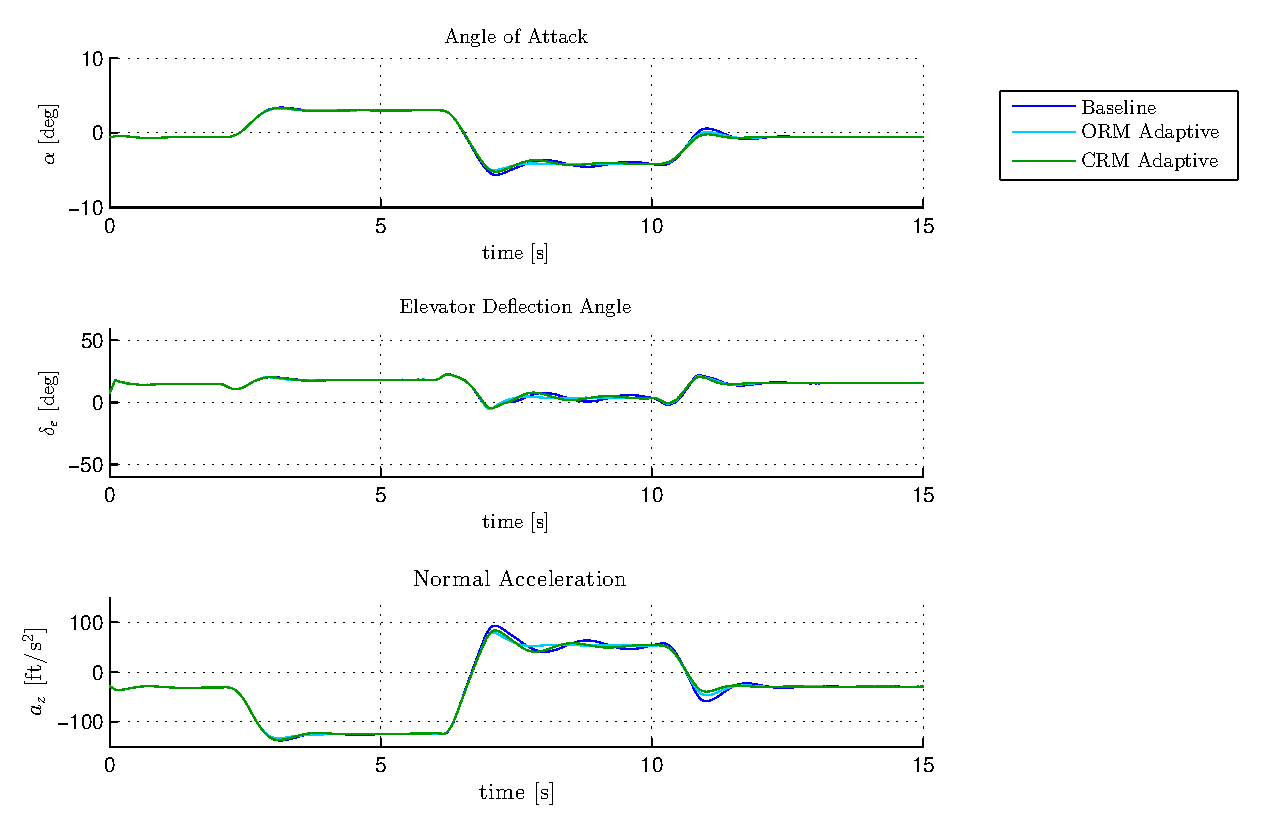
\includegraphics[width=5.0in]{\figurepath/select_longres_cef050b.eps}
    \caption{1A:\ 50\% control surface effectiveness on all surfaces}
  \end{center}
\end{figure}

\begin{figure}[H]
  \begin{center}
    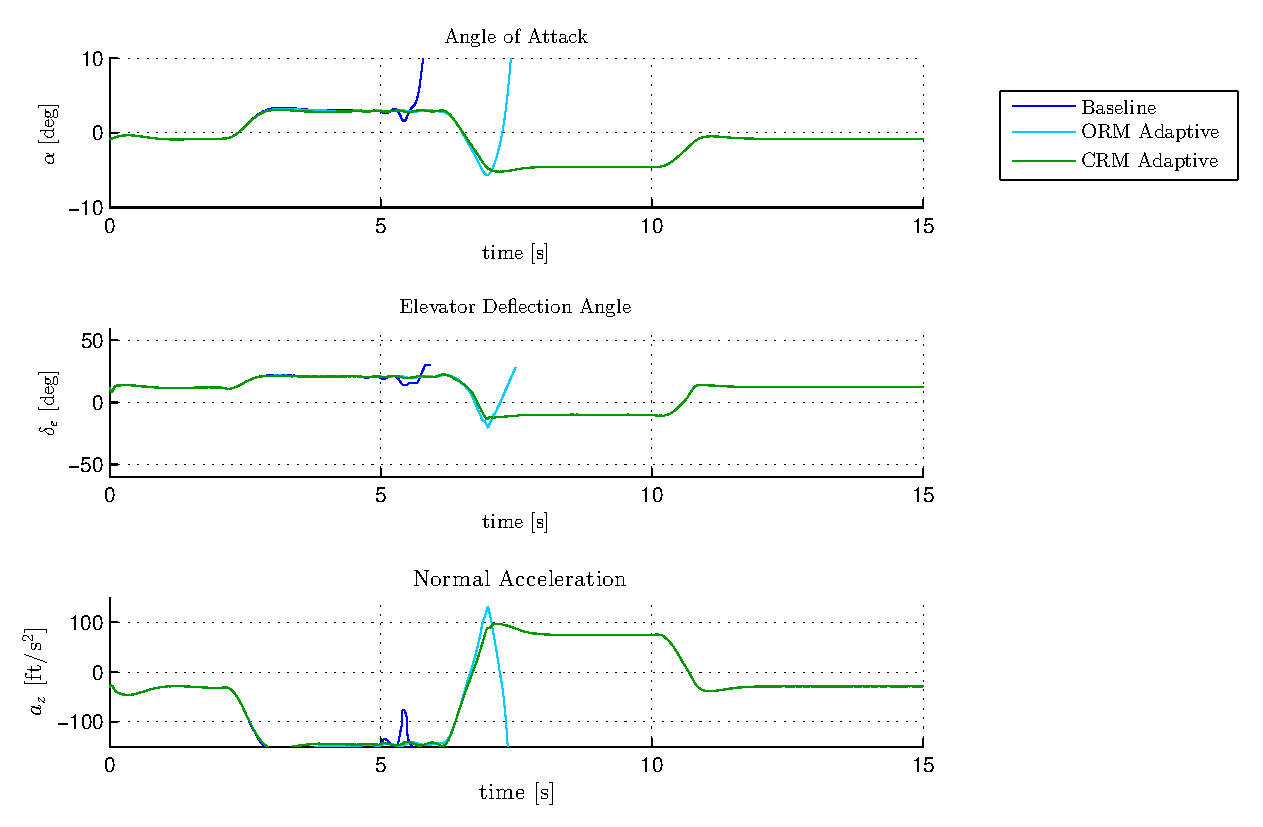
\includegraphics[width=5.0in]{\figurepath/select_longres_cgx090b.eps}
    \caption{1B:\ Longitudinal CG shift: -0.9 ft rearward}
  \end{center}
\end{figure}

\begin{figure}[H]
  \begin{center}
    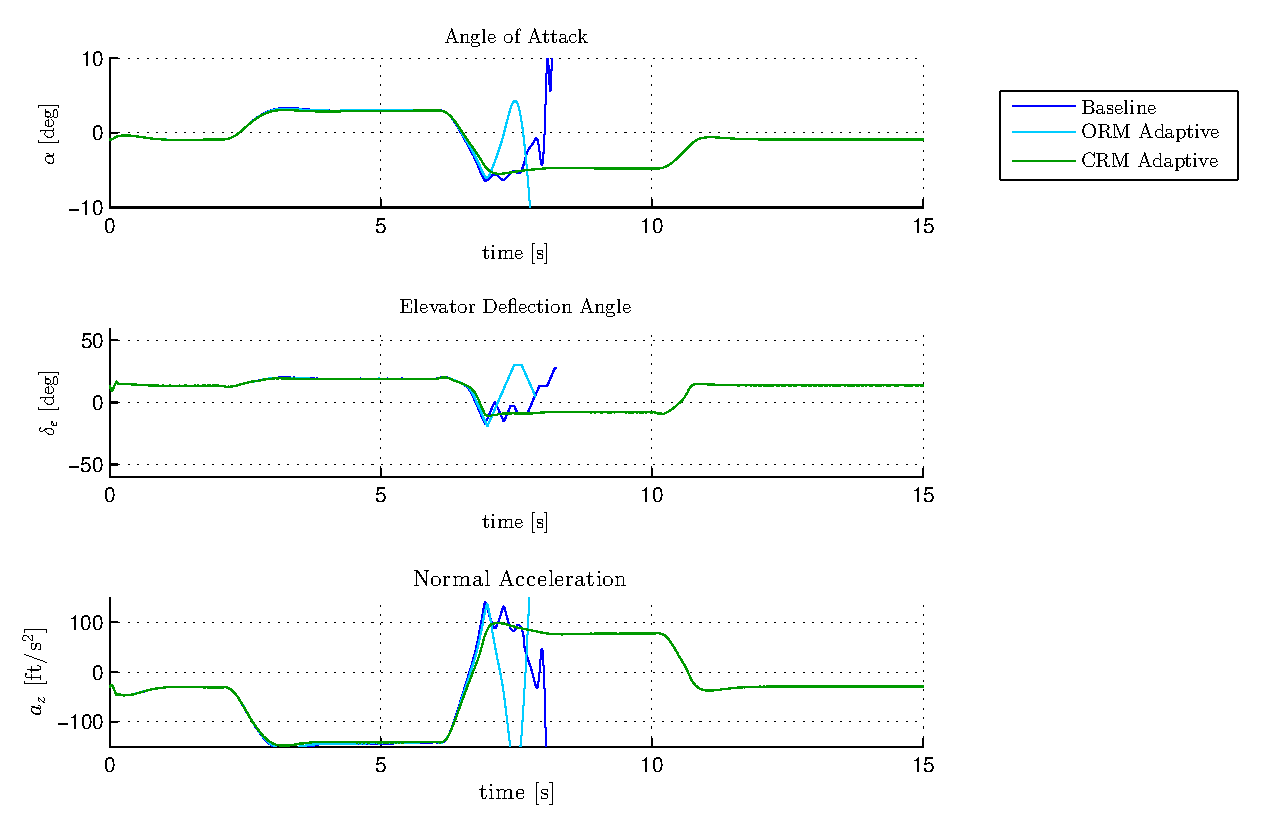
\includegraphics[width=5.0in]{\figurepath/select_longres_cma400b.eps}
    \caption{1C:\ Pitching moment coefficient $C_{m_{\alpha}}$ scaled $4\times$}
  \end{center}
\end{figure}

\begin{figure}[H]
  \begin{center}
    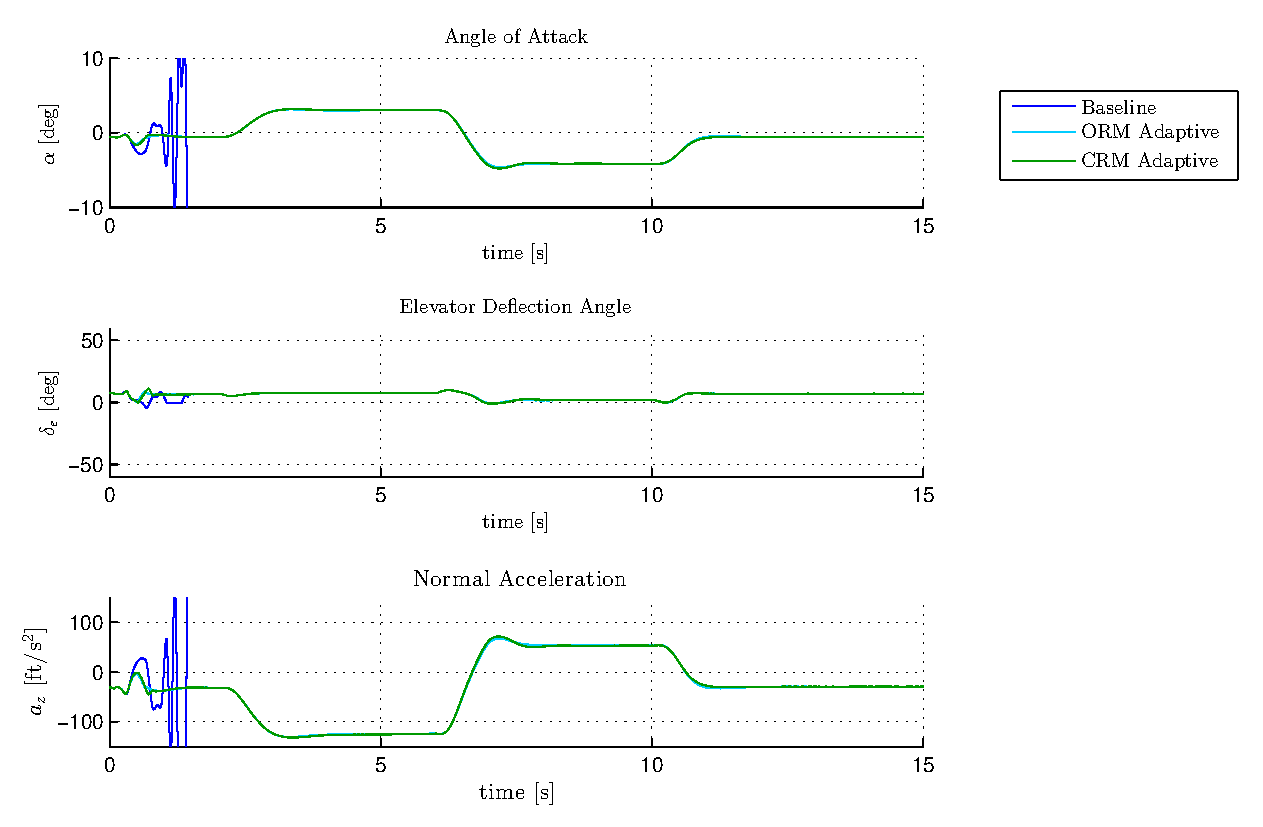
\includegraphics[width=4.9in]{\figurepath/select_longres_bia016b.eps}
    \caption{1D:\ Sensor bias of $+1.6$ degrees on sideslip measurement}
  \end{center}
\end{figure}

\subsection{Task 2: Roll Step}

\begin{figure}[H]
  \begin{center}
    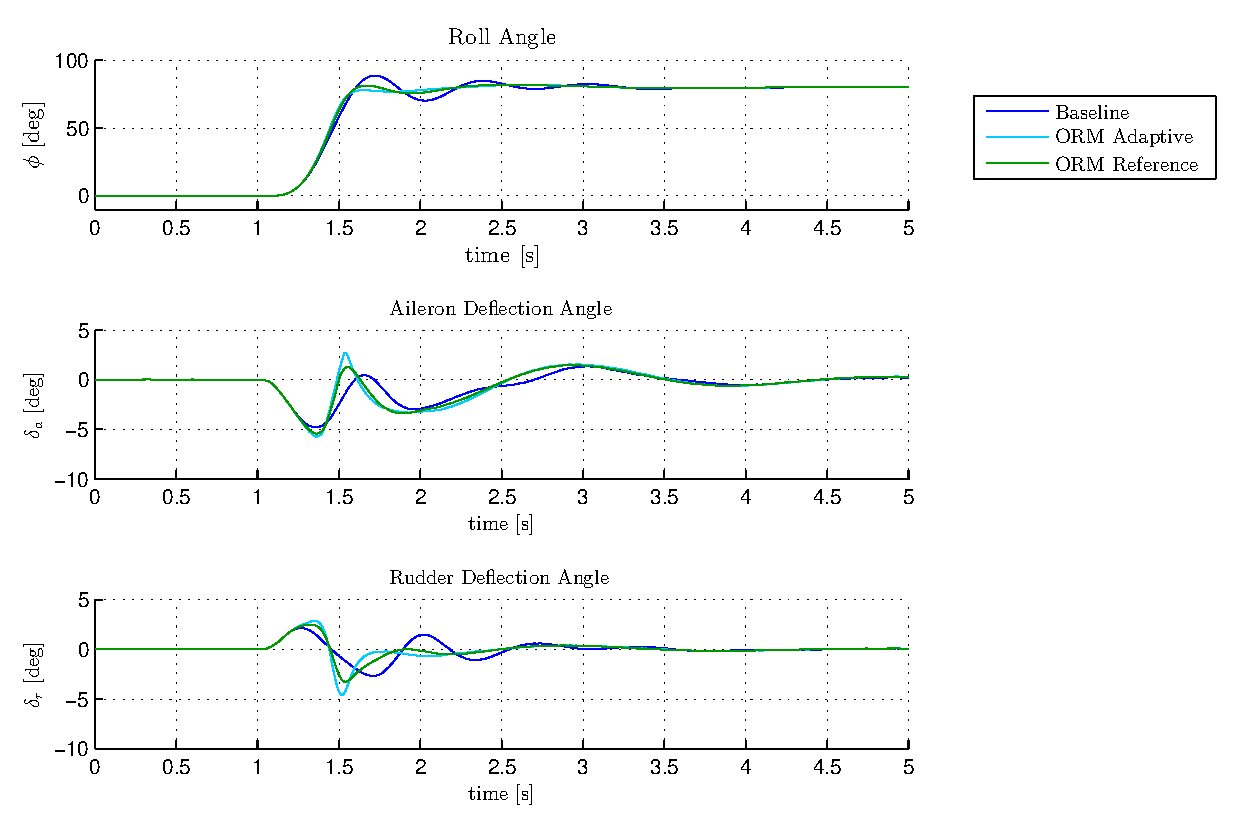
\includegraphics[width=4.9in]{\figurepath/select_latrres_cef050b.eps}
    \caption{2A:\ 50\% control surface effectiveness on all surfaces}
  \end{center}
\end{figure}

\begin{figure}[H]
  \begin{center}
    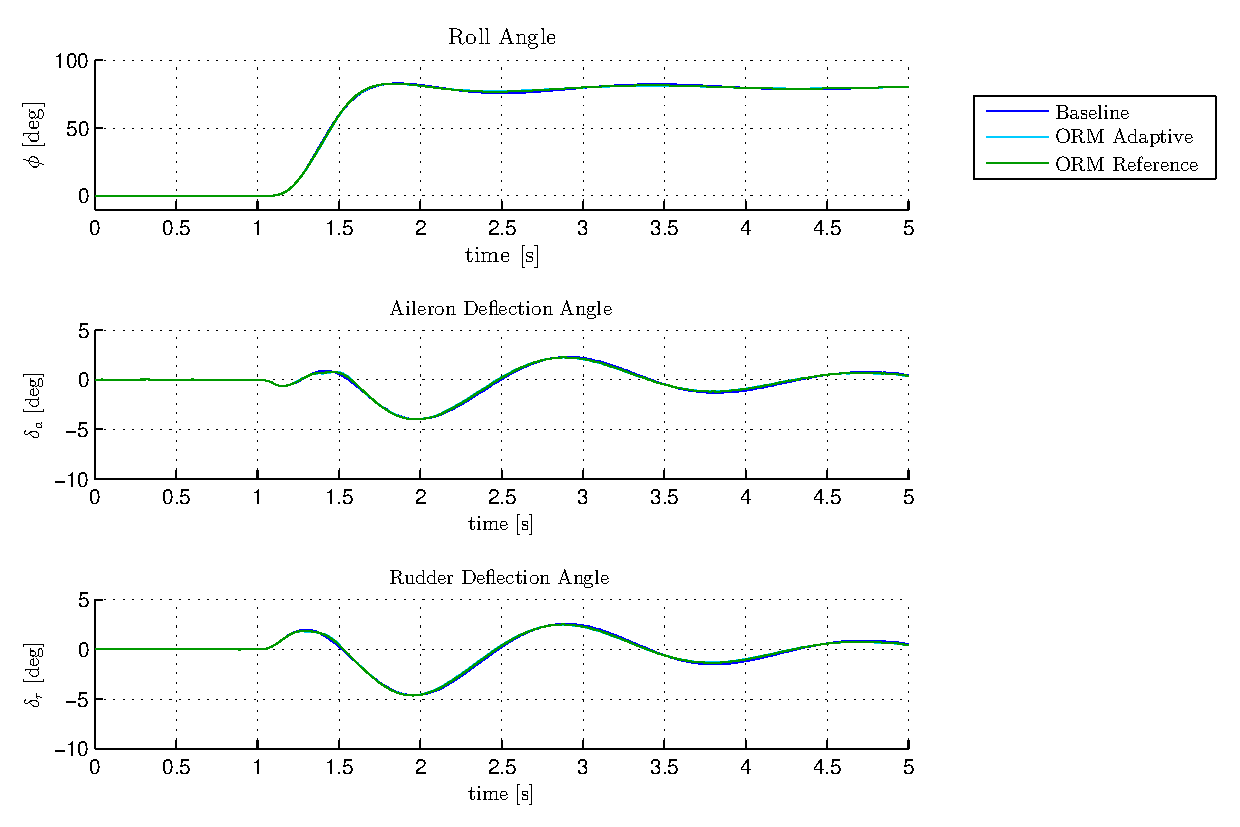
\includegraphics[width=4.9in]{\figurepath/select_latrres_cgx160b.eps}
    \caption{2B:\ Longitudinal CG shift: -1.6 ft rearward}
  \end{center}
\end{figure}

\begin{figure}[H]
  \begin{center}
    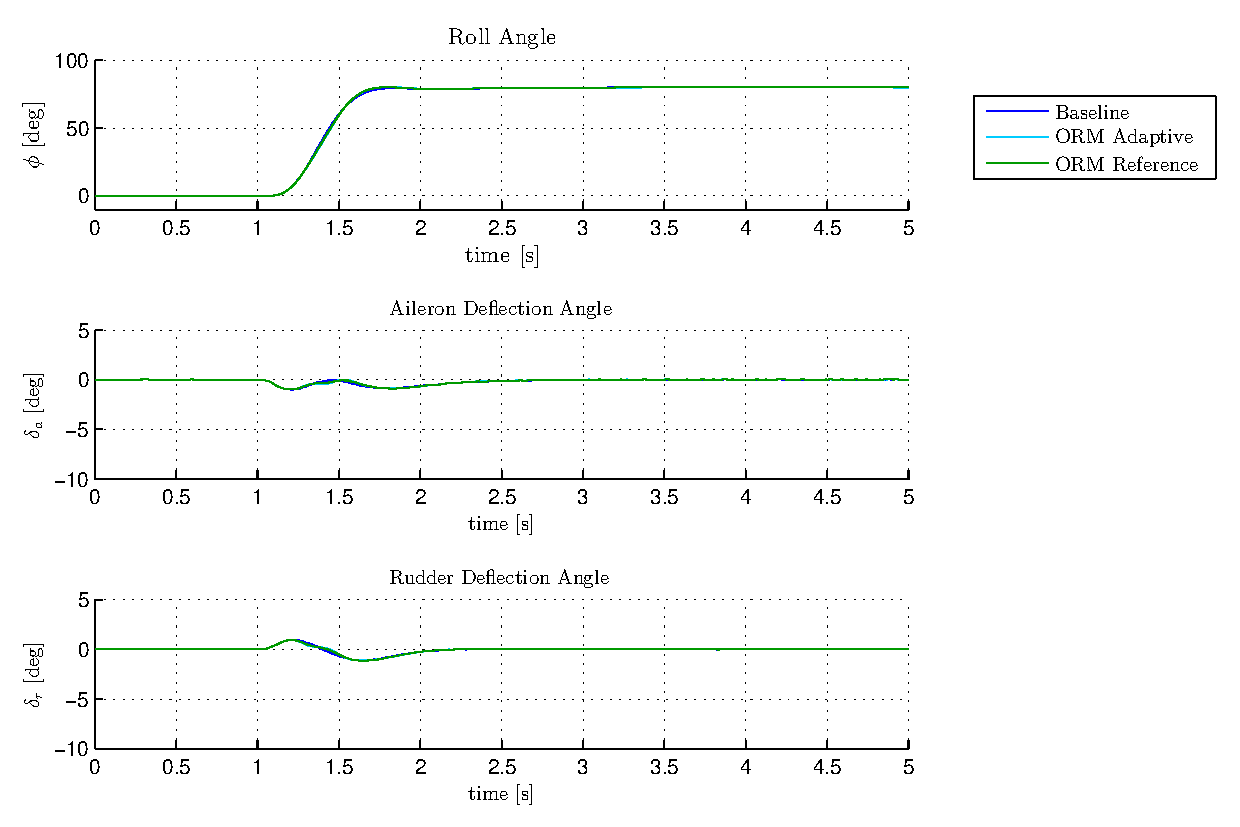
\includegraphics[width=5.0in]{\figurepath/select_latrres_cma400b.eps}
    \caption{2C:\ Pitching moment coefficient $C_{m_{\alpha}}$ scaled $4\times$}
  \end{center}
\end{figure}

\begin{figure}[H]
  \begin{center}
    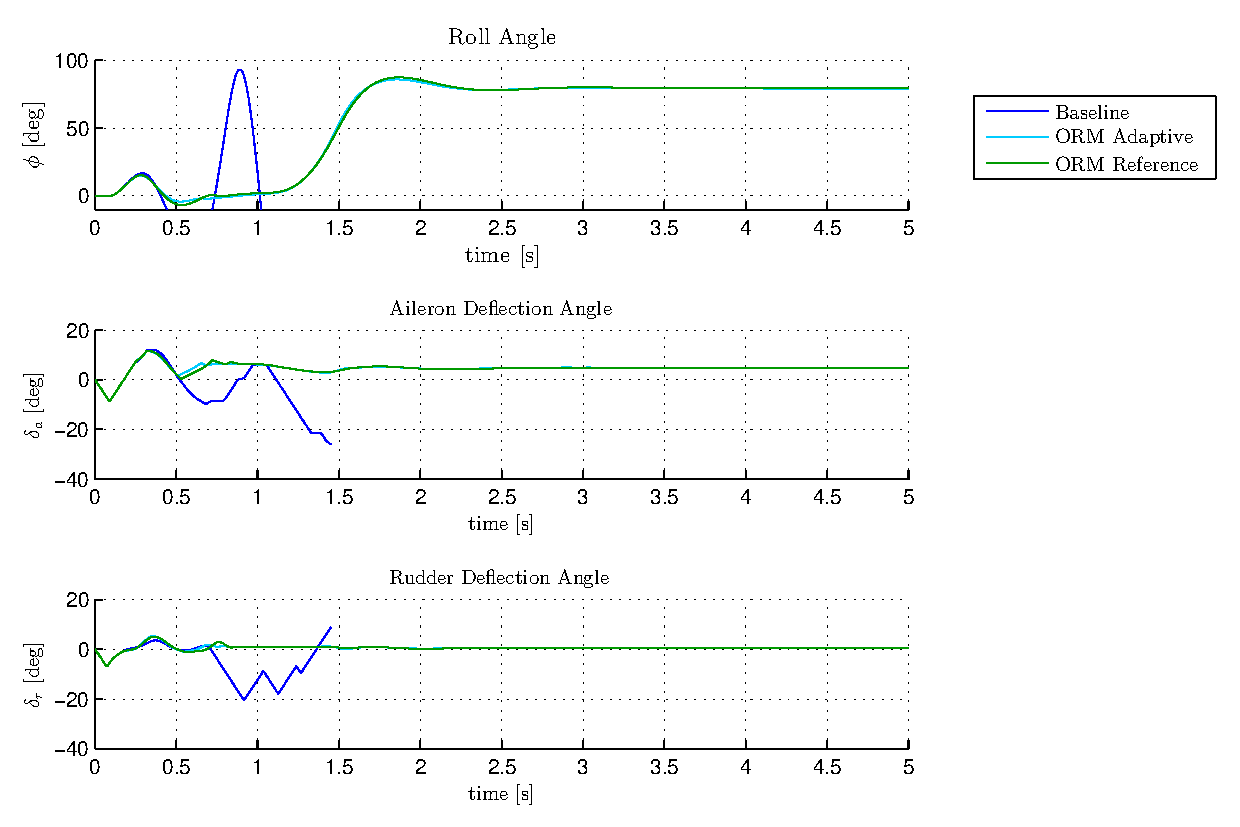
\includegraphics[width=5.0in]{\figurepath/select_latrres_bia016b.eps}
    \caption{2D:\ Sensor bias of $+1.6$ degrees on sideslip measurement}
  \end{center}
\end{figure}

In many of the cases presented here, the baseline controller is not able to maintain stability for the given task when subject to uncertainty.
Moreover, the ORM adaptive controller also is not able to maintain stability responses 1B and 1C, whereas the CRM adaptive controller is able to maintain stability.
For task 1, the CRM adaptive controller provides good closed-loop performance, with good transient response, minimal overshoot, almost no oscillations.
In response 1A, the baseline and ORM adaptive controller oscillate slightly more in the time response.
This behavior is even more pronounced as control effectiveness is reduced further, to the point where there is insufficient control authority to maintain stability.
In response 1B, the baseline and ORM adaptive controllers fail to maintain stability.
This is triggered by an oscillation in the lateral-directional dynamics, as can be seen in the full state plots in Appendix A.
However, the CRM adaptive controller maintains stability and good time response performance.
A similar situation is observed in response 1C, as the increased pitching moment coefficient has a very similar influence on the plant dynamics as a rearward CG shift.
In response 1D, the baseline controller becomes unstable very quickly, and both ORM and CRM adaptive controllers perform very well.

Response 2A shows the baseline controller again exhibiting significant oscillations in the time response when control effectiveness is reduced.
Both adaptive controllers significantly reduce this oscillation.
Minimal benefit of the adaptive controllers is observed in responses 2B and 2C, but this is largely due to the limited affect the longitudinal CG shift and pitching moment coefficient have on the lateral directional dynamics which are excited during the roll command.
Finally, response 1D again shows the baseline controller failing to maintain stability when subject to the sensor bias on the sideslip angle measurement.

\subsection{Time Delay Margins}

For some of the tasks and uncertainties demonstrated in simulation above, time delay margins were computed empirically for the three controllers by determining the maximum allowable input time delay that could be tolerated while maintaining stability.
Table~\ref{tab:delaymargins} shows the delay margins for each simulation result presented above.

\begin{table}[H]
  \centering
  \caption{Delay margins for selected responses in milliseconds\label{tab:delaymargins}}
  \small
  \begin{tabular}{lrrr}
    \toprule
    &\multicolumn{3}{c}{Controller} \\
    Response & Baseline & ORM & CRM \\
    \midrule
    1A & 33 & 36 & 41 \\
    1B & n/a & 3 & 18 \\
    1C & 26 & 19 & 19 \\
    2A & 34 & 13 & 26 \\
    \bottomrule
  \end{tabular}
\end{table}

While in the case of 1C and 2A, adaptation reduces the delay margin, all four cases show that the closed-loop reference model controller has a delay margin which is equal to or greater than the comparable open-loop reference model controller.
The delay margin of the CRM controller is at least 73\% that of the baseline controller, while the ORM controller has a delay margin which is as little as 38\% of that for the baseline controller.
Adaptation is required to maintain stability and provide good tracking performance, but must do so without sacrificing the delay margin to an unacceptable level.
The CRM adaptive controller is able to satisfy these requirements better than both the baseline and ORM adaptive controller.

\section{Summary}

In the simulation results presented above, the efficacy of the CRM adaptive controller was demonstrated on the GHV when performing two tasks while subject to four different uncertainties.
These uncertainties included decrease in control effectiveness, center-of-gravity shift, unknown pitching moment coefficient, and sensor bias on sideslip angle measurement.
In half of these cases, the baseline control design was not able to maintain stability, and in two cases the ORM adaptive controller failed.
The CRM adaptive controller maintained stability in all cases.
In addition, considering the cases where stable performance was maintained by the baseline and ORM adaptive controllers, the CRM adaptive showed improved time response behavior.
Finally, when a time delay was introduced at the control input, the CRM adaptive controller maintained a greater percentage of the time-delay margin provided by the baseline controller than the ORM adaptive controller did.
Overall, the CRM adaptive controller offers the best performance, tolerating a reduced control effectiveness of 50\%, rearward center of gravity shift of -0.9 to -1.6 feet (6--11\% of vehicle length), aerodynamic coefficient uncertainty scaled $4\times$ the nominal value, and sensor bias of $+1.6$ degrees on sideslip angle measurement.
The closed-loop reference model adaptive controller maintains at least 73\% of the delay margin provided by the robust baseline design, tolerating input time delays of between 18--46 ms during 3 degree angle of attack doublet, and 80 degree roll step commands.
These results demonstrate the necessity of an adaptive controller to provide stable and acceptable tracking performance, while still maintaining much of the delay margin provided by the robust baseline design.
